%\newpage
{\section{Wyniki i analiza pomiarów}}

{\subsection{Skalowanie termopary}}

\begin{figure}[!h]
    \centering
    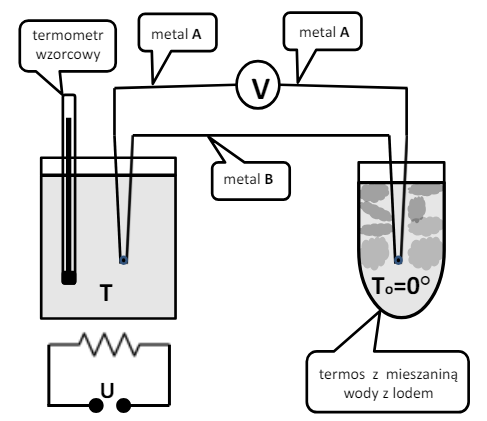
\includegraphics[width=8cm]{imgs/schemat_pom.png}
    \caption{Schemat pomiarowy}
    \label{fig:enter-label}
\end{figure}

\begin{center}
    \begin{tabular}{|c|c|}
        \hline
        Temperatura {[}$^{\circ}$C{]} & Napięcie {[}mV{]} \\ \hline \hline
        46                 & 46                \\ \hline
        48                 & 58                \\ \hline
        50                 & 65.3              \\ \hline
        52                 & 70.7              \\ \hline
        54                 & 75                \\ \hline
        56                 & 78.8              \\ \hline
        58                 & 81.6              \\ \hline
        60                 & 85.3              \\ \hline
        62                 & 89.2              \\ \hline
        64                 & 93.8              \\ \hline
    \end{tabular}
\end{center}

Wykres przedstawiający powyższe dane:
\begin{figure}[!ht]
    \centering
    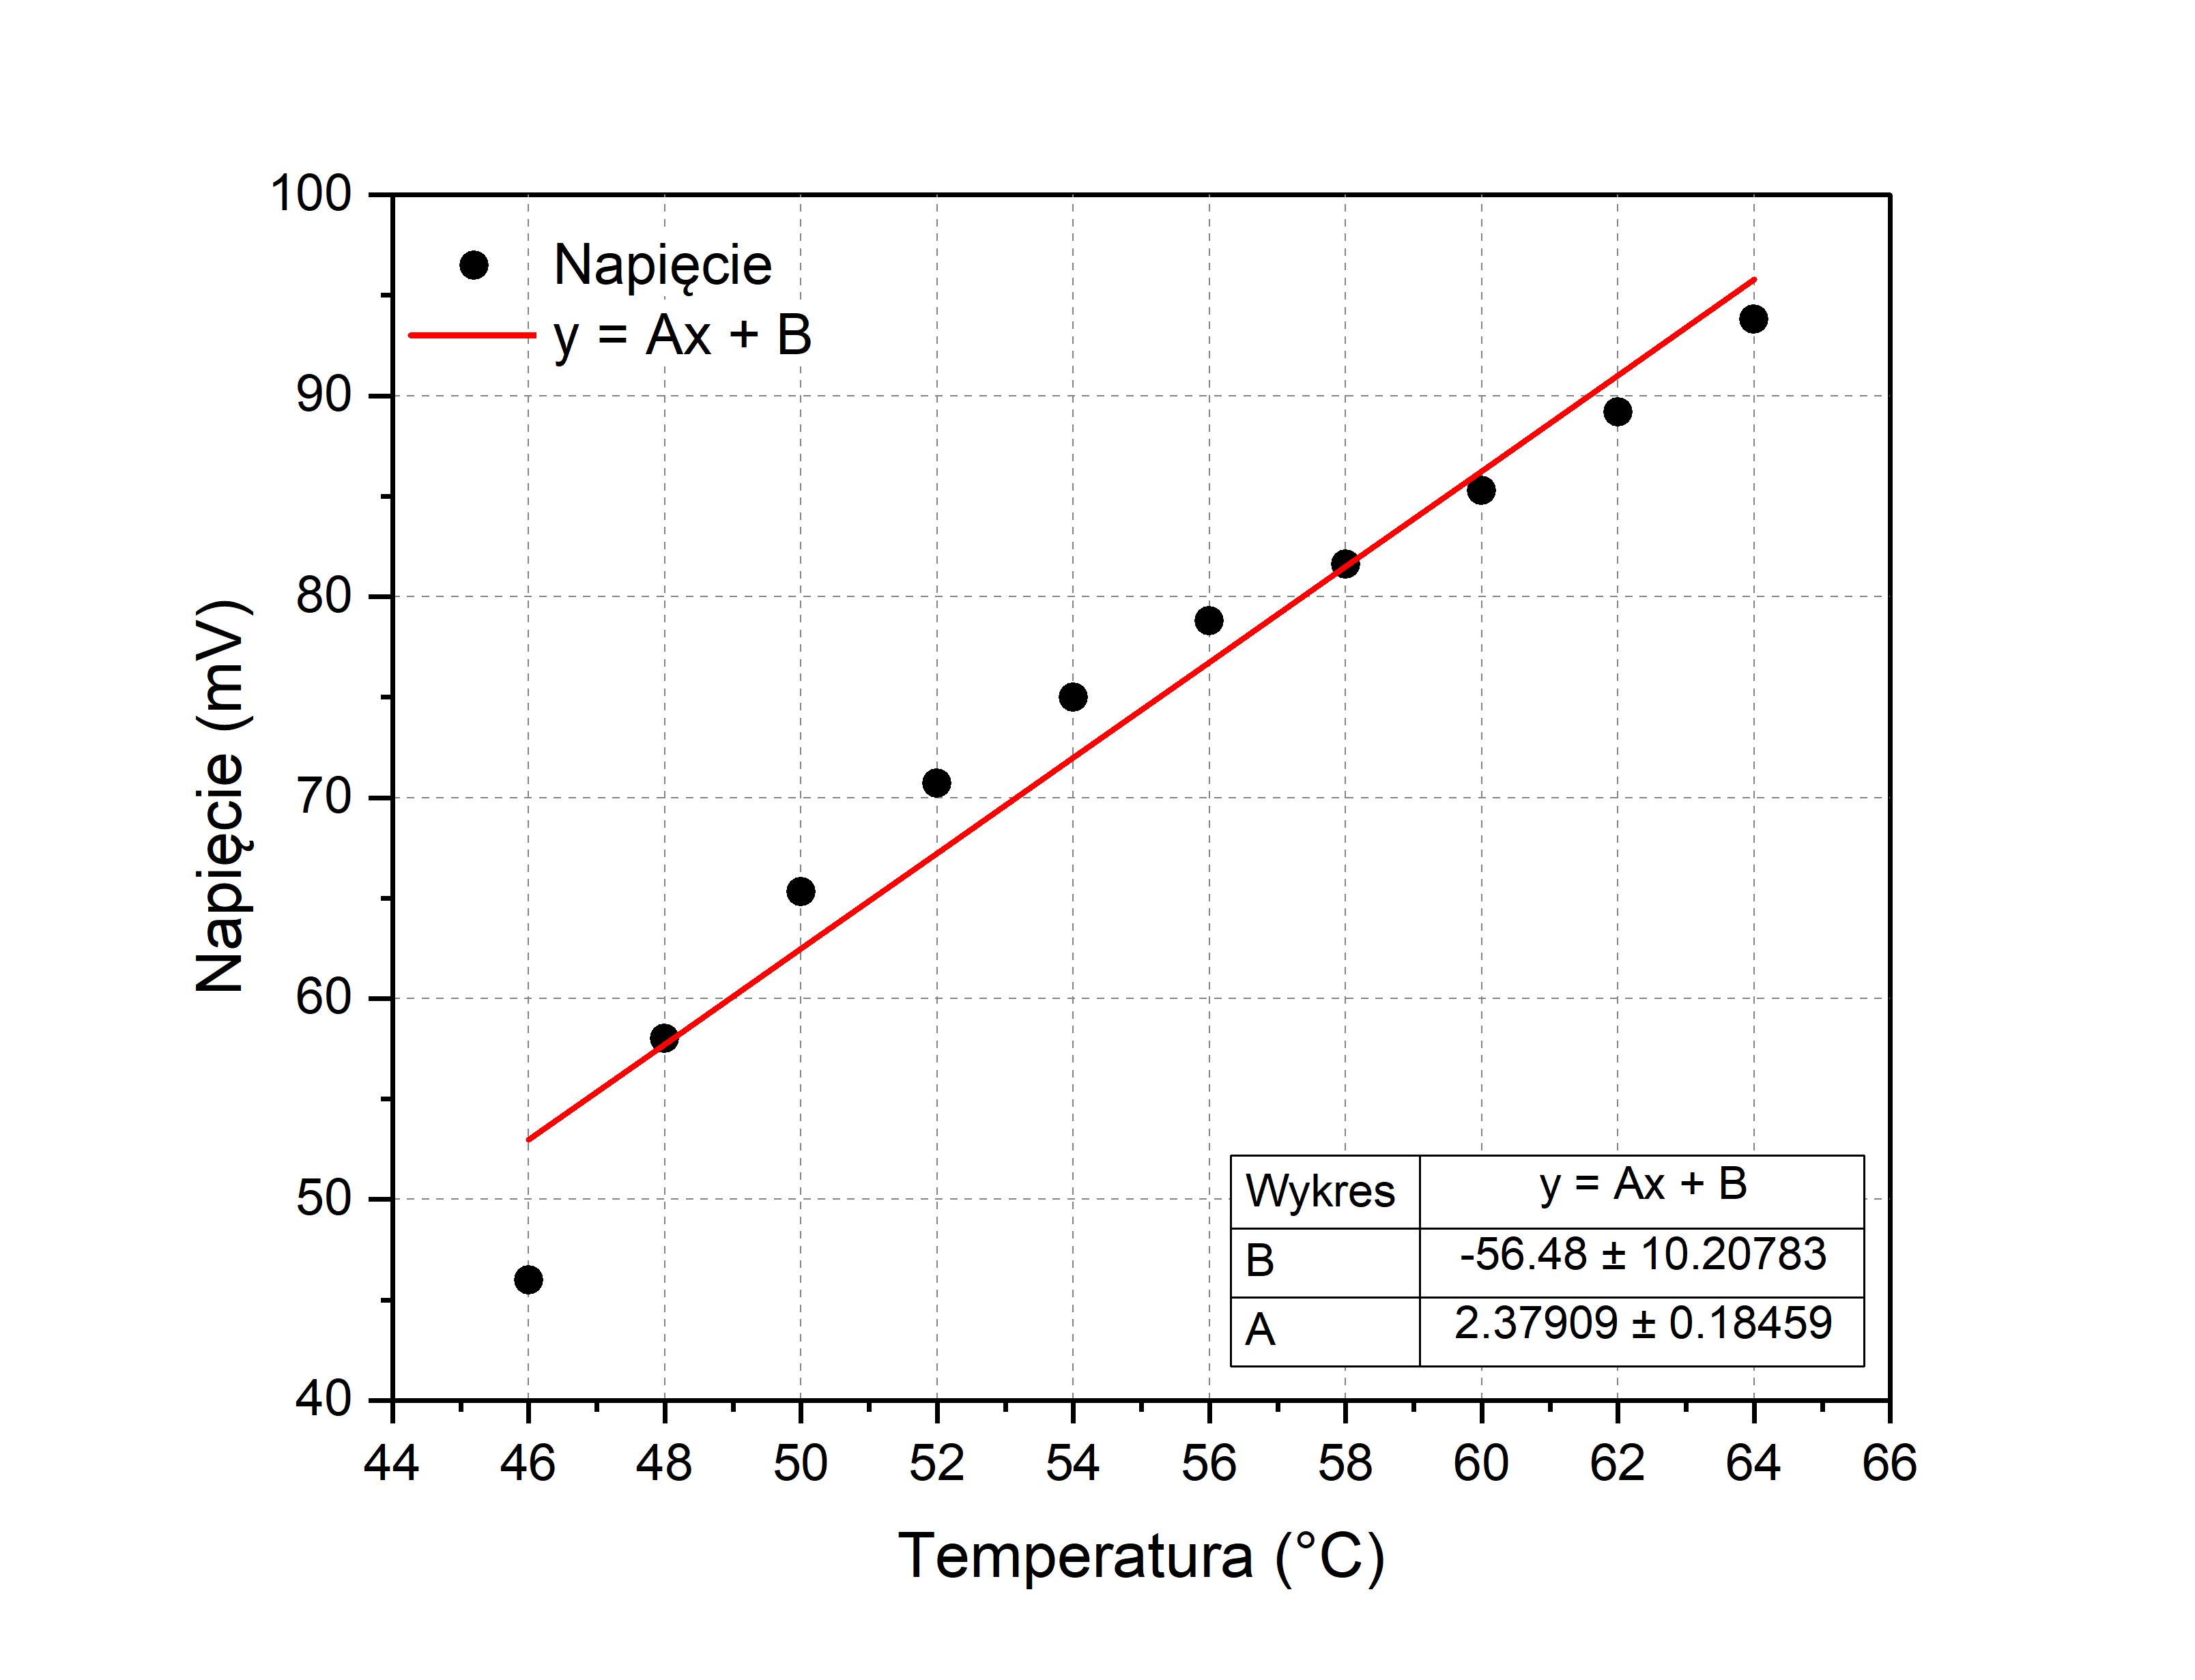
\includegraphics[width = 10cm]{imgs/Graph3.png}
    \caption{Wykres funkcji $U = f(T)$}
    \label{fig:wykres-skalowania}
\end{figure}

Dla powyższego wykresu możemy odczytać niepewność współczynnika kierunkowego u(A), który równa się: $$u(A) = u(\alpha) \approx 0.1846$$

\newpage % Bo wykres renderuje się w złym miejscu
{\subsection{Wyznaczenie temperatury krzepnięcia wody oraz niepewności jej wyznaczenia}}

% Tabela wyników pomiarów
\begin{multicols}{3}
    \begin{center}
        \begin{tabular}{|c|c|}
            \hline
            Czas {[}s{]} & Napięcie {[}V{]} \\ \hline \hline
            0            & -0.823           \\ \hline
            20           & -0.8188          \\ \hline
            40           & -0.825           \\ \hline
            60           & -0.853           \\ \hline
            80           & -0.8754          \\ \hline
            100          & -0.896           \\ \hline
            120          & -0.8986          \\ \hline
            140          & -0.8996          \\ \hline
            160          & -0.893           \\ \hline
            180          & -0.8997          \\ \hline
            200          & -0.918           \\ \hline
            220          & -0.938           \\ \hline
            240          & -0.958           \\ \hline
            260          & -0.9865          \\ \hline
            280          & -0.977           \\ \hline
            300          & -0.966           \\ \hline
            320          & -0.993           \\ \hline
            340          & -0.955           \\ \hline
            360          & -0.9826          \\ \hline
            380          & -0.977           \\ \hline
        \end{tabular}
        \begin{tabular}{|c|c|}
            \hline
            Czas {[}s{]} & Napięcie {[}V{]} \\ \hline \hline
            400          & -0.9949          \\ \hline
            420          & -1.0113          \\ \hline
            440          & -1.0064          \\ \hline
            460          & -1.0094          \\ \hline
            480          & -1.0144          \\ \hline
            500          & -1.0119          \\ \hline
            520          & -1.0216          \\ \hline
            540          & -1.023           \\ \hline
            560          & -1.038           \\ \hline
            580          & -1.039           \\ \hline
            600          & -1.075           \\ \hline
            620          & -1.1111          \\ \hline
            640          & -1.1352          \\ \hline
            660          & -1.1556          \\ \hline
            680          & -1.1654          \\ \hline
            700          & -1.18            \\ \hline
            720          & -1.146           \\ \hline
            740          & -1.1364          \\ \hline
            760          & -1.1468          \\ \hline
            780          & -1.165           \\ \hline
        \end{tabular}
        \begin{tabular}{|c|c|}
            \hline
            Czas {[}s{]} & Napięcie {[}V{]} \\ \hline \hline
            800          & -1.174           \\ \hline
            820          & -1.164           \\ \hline
            840          & -1.136           \\ \hline
            860          & -1.124           \\ \hline
            880          & -1.1278          \\ \hline
            900          & -1.1286          \\ \hline
            920          & -1.116           \\ \hline
            940          & -1.1186          \\ \hline
            960          & -1.1236          \\ \hline
            980          & -1.1203          \\ \hline
            1000         & -1.1332          \\ \hline
            1020         & -1.1338          \\ \hline
            1040         & -1.122           \\ \hline
            1060         & -1.122           \\ \hline
            1080         & -1.118           \\ \hline
            1100         & -1.111           \\ \hline
            1120         & -1.145           \\ \hline
            1140         & -1.164           \\ \hline
            1160         & -1.159           \\ \hline
        \end{tabular}
    \end{center}
\end{multicols} \vspace{3mm}

Wykres przedstawiający powyższe dane:
\begin{figure}[!ht]
    \centering
    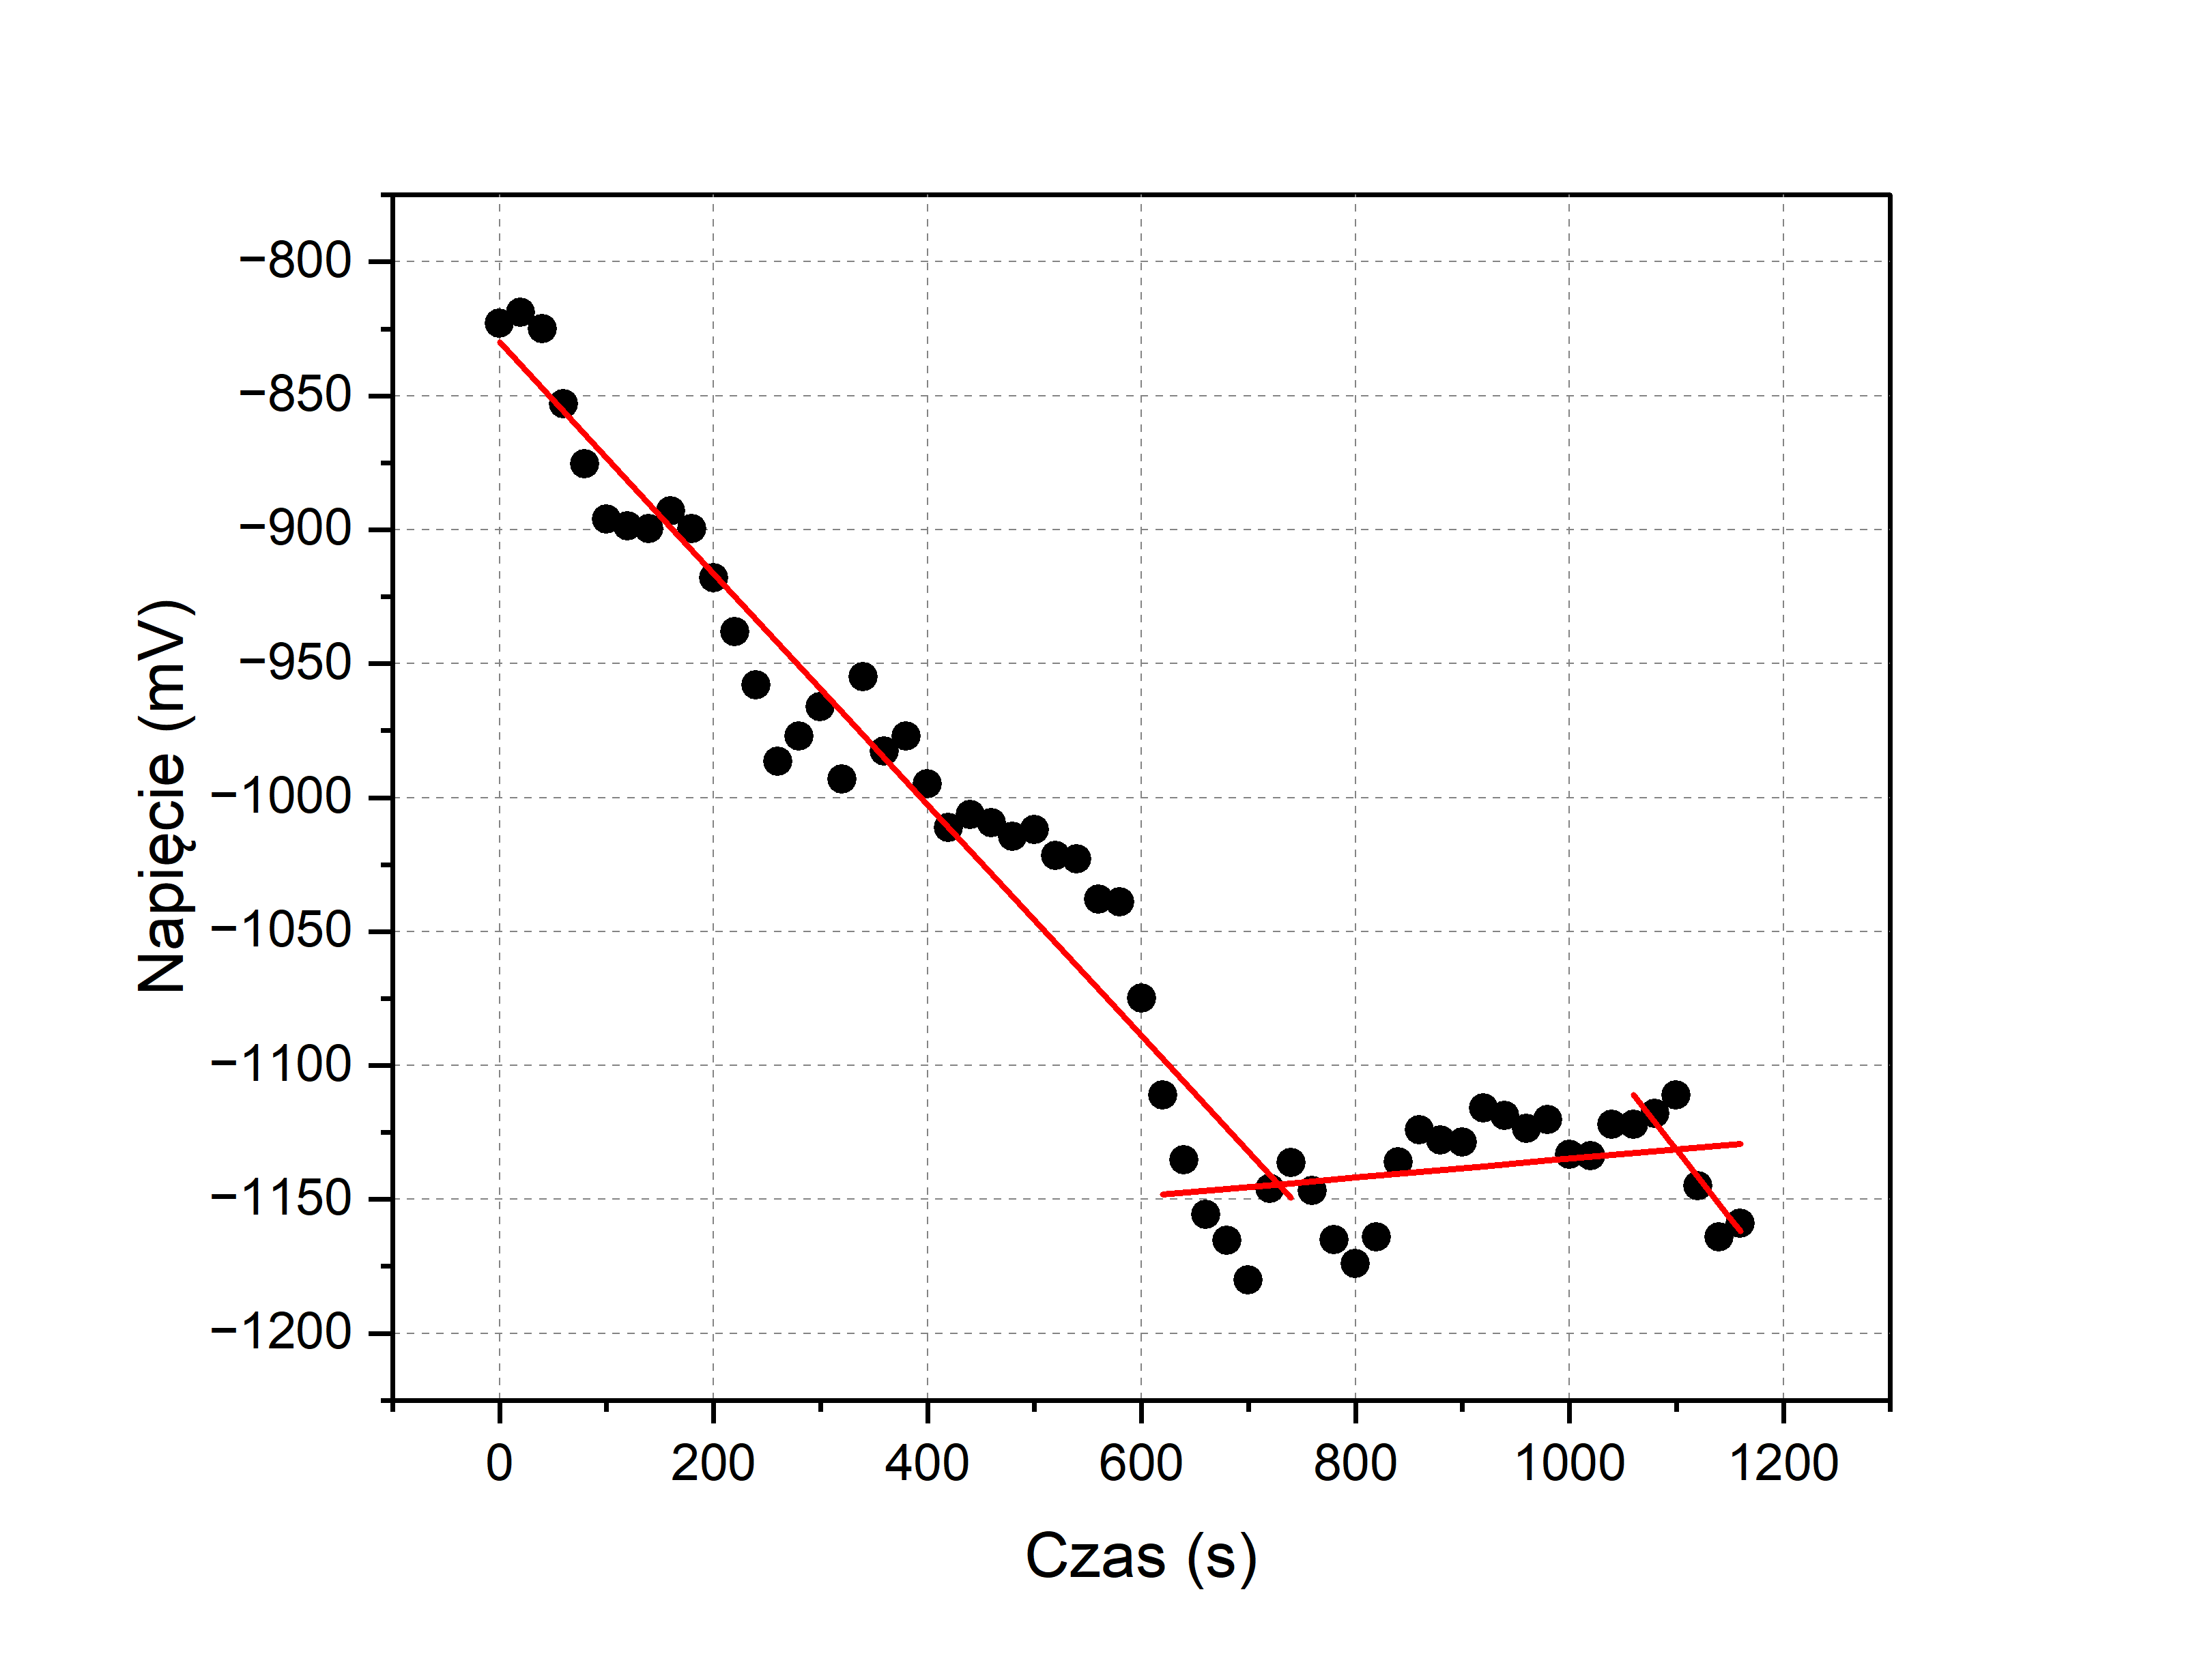
\includegraphics[width = 9cm]{imgs/Graph5.png}
    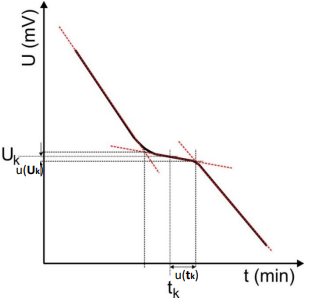
\includegraphics[width = 6cm]{imgs/graph4.png}
    \caption{Wykres funkcji $U = f(t)$, oraz wyznaczanie wartości $U_k$ oraz niepewności u($U_k$)}
    \label{fig:wykres-krzepniecie}
\end{figure}
% ======================
$$ U_k=-1.1373mV $$

Aby obliczyć niepewność u($U_k$) nusimy najpierw policzyć niepewność standardową średniej napięć w obszarze plateau:

\begin{equation*}
    \displaystyle u_A(\overline{U}) = \sqrt{ \frac{ \displaystyle \sum_{i=1}^{n} (U_i - \overline{U} )^2 }{ n(n - 1) } }= 0.005380
\end{equation*} \\

Następnie liczymy niepewność typu B:

\begin{equation*}
    \displaystyle u_B(x) = \sqrt{ \frac{ (\Delta_p U)^2 }{3} }=0.00005774
\end{equation*} \\

Na końcu możemy policzyć niepewność całkowitą u($U_k$):

\begin{equation*}
    \displaystyle u(x) = \sqrt{ u_A^2 + u_B^2 }=0.00544
\end{equation*}

Po analizie powyższych danych z wykresu jesteśmy w stanie wyznaczyć temperaturę krzepnięcia wody: \\

\begin{equation*}
    T_k=\frac{U_k+B}{\alpha}=\frac{-1.1373-56.48}{2.3791} \approx -24.218 ^{\circ}C \approx -24 ^{\circ}C
\end{equation*} \\

Niepewność złożona $u_c(T_k)$ będzie równa:

\begin{equation*}
    \begin{aligned}
        u_c^2(T_k(U_k, B, \alpha)) &= \displaystyle\sum_{i=1}^{n} \left( \frac{\partial f}{\partial x_i} \right)^2 u^2(x_i)
        = \left( \frac{1}{\alpha} \right)^2 \cdot u^2(U_k) + \left( \frac{1}{\alpha} \right)^2 \cdot u^2(B) + \left( -\frac{U_k + B}{\alpha^2} \right)^2 \cdot u^2(\alpha) \\
        &= \left( \frac{1}{2.3791} \right)^2 \cdot (0.00538)^2 + \left( \frac{1}{2.3791} \right)^2 \cdot (10.2078)^2 + \left( -\frac{-1.1373 - 56.48}{(2.3791)^2} \right)^2 \cdot (0.1846)^2 
        \approx 4.6841^{\circ}C
    \end{aligned}
\end{equation*} \\